% Autor: Leonhard Segger, Alexander Neuwirth
% Datum: 2017-10-30
\documentclass[
	% Papierformat
	a4paper,
	% Schriftgröße (beliebige Größen mit „fontsize=Xpt“)
	12pt,
	% Schreibt die Papiergröße korrekt ins Ausgabedokument
	pagesize,
	% Sprache für z.B. Babel
	ngerman
]{scrartcl}

% Achtung: Die Reihenfolge der Pakete kann (leider) wichtig sein!
% Insbesondere sollten (so wie hier) babel, fontenc und inputenc (in dieser
% Reihenfolge) als Erstes und hyperref und cleveref (Reihenfolge auch hier
% beachten) als Letztes geladen werden!

% Silbentrennung etc.; Sprache wird durch Option bei \documentclass festgelegt
\usepackage{babel}
% Verwendung der Zeichentabelle T1 (Sonderzeichen etc.)
\usepackage[T1]{fontenc}
% Legt die Zeichenkodierung der Eingabedatei fest, z.B. UTF-8
\usepackage[utf8]{inputenc}
% Schriftart
\usepackage{lmodern}
% Zusätzliche Sonderzeichen
\usepackage{textcomp}

% Mathepaket (intlimits: Grenzen über/unter Integralzeichen)
\usepackage[intlimits]{amsmath}
% Ermöglicht die Nutzung von \SI{Zahl}{Einheit} u.a.
\usepackage{siunitx}
% Zum flexiblen Einbinden von Grafiken (\includegraphics)
\usepackage{graphicx}
% Abbildungen im Fließtext
\usepackage{wrapfig}
% Abbildungen nebeneinander (subfigure, subtable)
\usepackage{subcaption}
% Funktionen für Anführungszeichen
\usepackage{csquotes}
% Zitieren, Bibliographie
\usepackage{biblatex}

% Verlinkt Textstellen im PDF-Dokument
\usepackage[unicode]{hyperref}
% "Schlaue" Referenzen (nach hyperref laden!)
\usepackage{cleveref}
% Zur Darstellung von Webadressen
\usepackage{url}
%chemische Formeln
\usepackage[version=4]{mhchem}
% siunitx: Deutsche Ausgabe, Messfehler getrennt mit ± ausgeben
\usepackage{floatrow}
\floatsetup[table]{capposition=top}
\sisetup{
	locale=DE,
	separate-uncertainty
}
%\bibliography{6Mi_S2_25-10-2017_References}

\begin{document}
	
	\begin{titlepage}
		\centering
		{\scshape\LARGE Versuchsbericht zu \par}
		\vspace{1cm}
		{\scshape\huge M1 - Drehpendel nach Pohl\par}
		\vspace{2.5cm}
		{\LARGE Gruppe 6Mi \par}
		\vspace{0.5cm}
		
		{\large Alexander Neuwirth (E-Mail: a\_neuw01@wwu.de) \par}
		{\large Leonhard Segger (E-Mail: l\_segg03@uni-muenster.de) \par}
		\vfill
		
		durchgeführt am 21.11.2017\par
		betreut von\par
		{\large Torsten Stiehm}
		
		\vfill
		
		{\large \today\par}
	\end{titlepage}
	\tableofcontents
	\newpage
	
	\section{Kurzfassung}
	Das Drehpendel nach Pohl ist ein Beispiel für schwingfähige Systeme.
	\section{Methoden}
	
	\subsection{Drehpendel ohne Dämpfung}%...
	Zunächst haben wir, um die Eigenfrequenz des Drehpendels (annähernd) ohne Dämpfung zu bestimmen, erst mithilfe einer Stoppuhr die Periodendauer bestimmt. Um den Fehler, der durch die menschliche Reaktionszeit entsteht, zu minimieren, haben wir die Zeit, die das Drehpendel für 20 Schwingungen benötigt, gemessen, um dann über diese zu mitteln.
	Als Anfangs- und Endpunkt der Messung haben wir die Ruhelage der Scheibe gewählt, da sie sich an dieser Stelle mit näherungsweise konstanter Geschwindigkeit bewegt und man somit den Reaktionsfehler leichter ausgleichen kann.
	Alternativ hätte man den linken oder rechten Wendepunkt der Bewegung wählen können. An dieser Stelle bewegt sich das Pendel allerdings langsam und der Zeitraum, in dem das Pendel stillsteht, ist groß, weshalb das Ende der Bewegung schwer exakt zu erkennen ist. %Von sich selbst darf man ja wohl plagiarisieren.
	Dann haben wir dieselbe Messung erneut durchgeführt, diesmal allerdings als Messkurve mit dem Computer aufgezeichnet, wozu das Schwingrad über einen Faden mit einem Messrad, dessen Drehung digital erfasst werden konnte, verbunden wurde. %Cyber Cyber
	\subsection{Drehpendel mit Dämpfung}
	Im Anschluss daran fügten wir eine Dämpfung in Form einer Wirbelstrombremse hinzu. Von dem sich ergebenden Schwingungsvorgang haben wir drei Messkurven mit jeweils unterschiedlichen Dämpfungen, also unterschiedlichem Stromfluss durch die Spulen der Wirbelstrombremse, aufgenommen. Hieraus konnten wir die jeweils die Eigenfrequenz und die Dämpfung aus der Abnahme der Amplitude bestimmen. %Sollte man hier die konkreten Werte des Stromflusses nennen? Denke nicht.
	\subsection{Drehpendel mit Exzenter und Dämpfung} 
	Nun haben wir das Drehpendel mit einem Exzenter (in Form eines Motors, der die Spiralfeder ansteuert) und der Wirbelstrombremse betrieben. Hierbei haben wir darauf geachtet die Messung erst zu starten, nachdem das Pendel die Einschwingphase überwunden hatte, also sich Frequenz und Amplitude nicht mehr merklich änderten.
	Zunächst nahmen wir eine Kalibrierkurve auf, um den Zusammenhang zwischen der Frequenz der Anregung $\omega$ und der Spannung am Tacho-Ausgang des Motors zu quantifizieren.
	Anschließend haben wir für drei verschiedene Dämpfungen je 20 Messungen mit unterschiedlicher Anregungsfrequenz $\omega$ durchgeführt. Gemessen wurde jeweils für ca. \SI{20}{\second}. 
	\subsection{Qualitative Beobachtungen und Vergleich zum Fadenpendel}
	Wir haben bei kleiner Dämpfung den Phasenunterschied zwischen Anregung und Drehpendel bei Frequenzen über, unter und nahe bei der Resonanzfrequenz beobachtet. Dann haben wir dieselbe Untersuchung bei einem Fadenpendel durchgeführt, um die Parallelen erkennen zu können.
	\subsection{Einführung einer Nichtlinearität}
	Zuletzt wurde noch eine Nichtlinearität in Form eines kleinen Gewichtes eingeführt. Diese Gewicht haben wir am oberen Rand der Scheibe (eine Daumenbreite neben dem obersten Punkt) in Ruhelage befestigt. Dann haben wir das Verhalten des Drehpendels bei steigender sowie bei sinkender Anregungsfrequenz beobachtet. Anschließend haben wir näherungsweise die Resonanzfrequenz eingestellt und die Schwingung beobachtet.
	
	\section{Ergebnisse und Diskussion}
	
	\subsection{Drehpendel ohne Dämpfung}
	Die Messung mit einer Stoppuhr ergibt eine Dauer von $T_20 =\SI{28,15}{\second}$ für 20 Schwingungen, also pro Schwingung $ T_\text{Uhr} = \SI{1,41}{\second}$. %TODO seltsame Underfull hbox Warnung
	Für die Unsicherheit von \(T\) gilt: \\
	\begin{itemize}
		\item  Digitalanzeige der Stoppuhr \SI{\pm 0,005}{\second}, (Typ B): \( u_B(T) = \frac{2\cdot \SI{0,005}{\second}}{2 \cdot 20 \sqrt{3}} = \SI{0,00014}{\second} \)
		\item Reaktionszeit \SI{\pm 0,1}{\second}, (Typ B): \( u_B(T) \approx \frac{2\cdot \SI{0,1}{\second}}{2 \cdot 20 \sqrt{3}} = 0.0029\si{s} \)
		\item Komb. Unsicherheit: $ u_\text{Uhr}(T) = \sqrt{(0,00014\si{s})^2+(0.0029\si{s})^2} \approx 0,0029 \si{s} $
	\end{itemize} 
	$ \implies T_\text{Uhr} = \SI{1,41 \pm 0,0029}{\second} $ \newline 
	Für die Frequenz ergibt sich daraus $ f_\text{Uhr} = \frac{1}{T_\text{Uhr}} = \SI{0,71}{\per \second}$ und für die Unsicherheit: \newline
	
	\begin{equation}
		u_\text{Uhr}(f) = \left|  \frac{\partial f}{\partial T_\text{Uhr}} u_\text{Uhr}(T_\text{Uhr}) \right| = \left| - \frac{1}{T_\text{Uhr}^2}u_\text{Uhr}(T_\text{Uhr}) \right| \approx \SI{0,0015}{\per \second} %Ich hoffe mal das ist rechnerisch richtig, man könnte sich beschweren, dass wir bei der Unsicherheit mehr Stellen von f,t,u angeben müssten
	\end{equation}
	Insgesamt: $f_\text{Uhr} = \SI{0,71 \pm 0,0015}{\per \second}  $
	\begin{figure}[htb]
		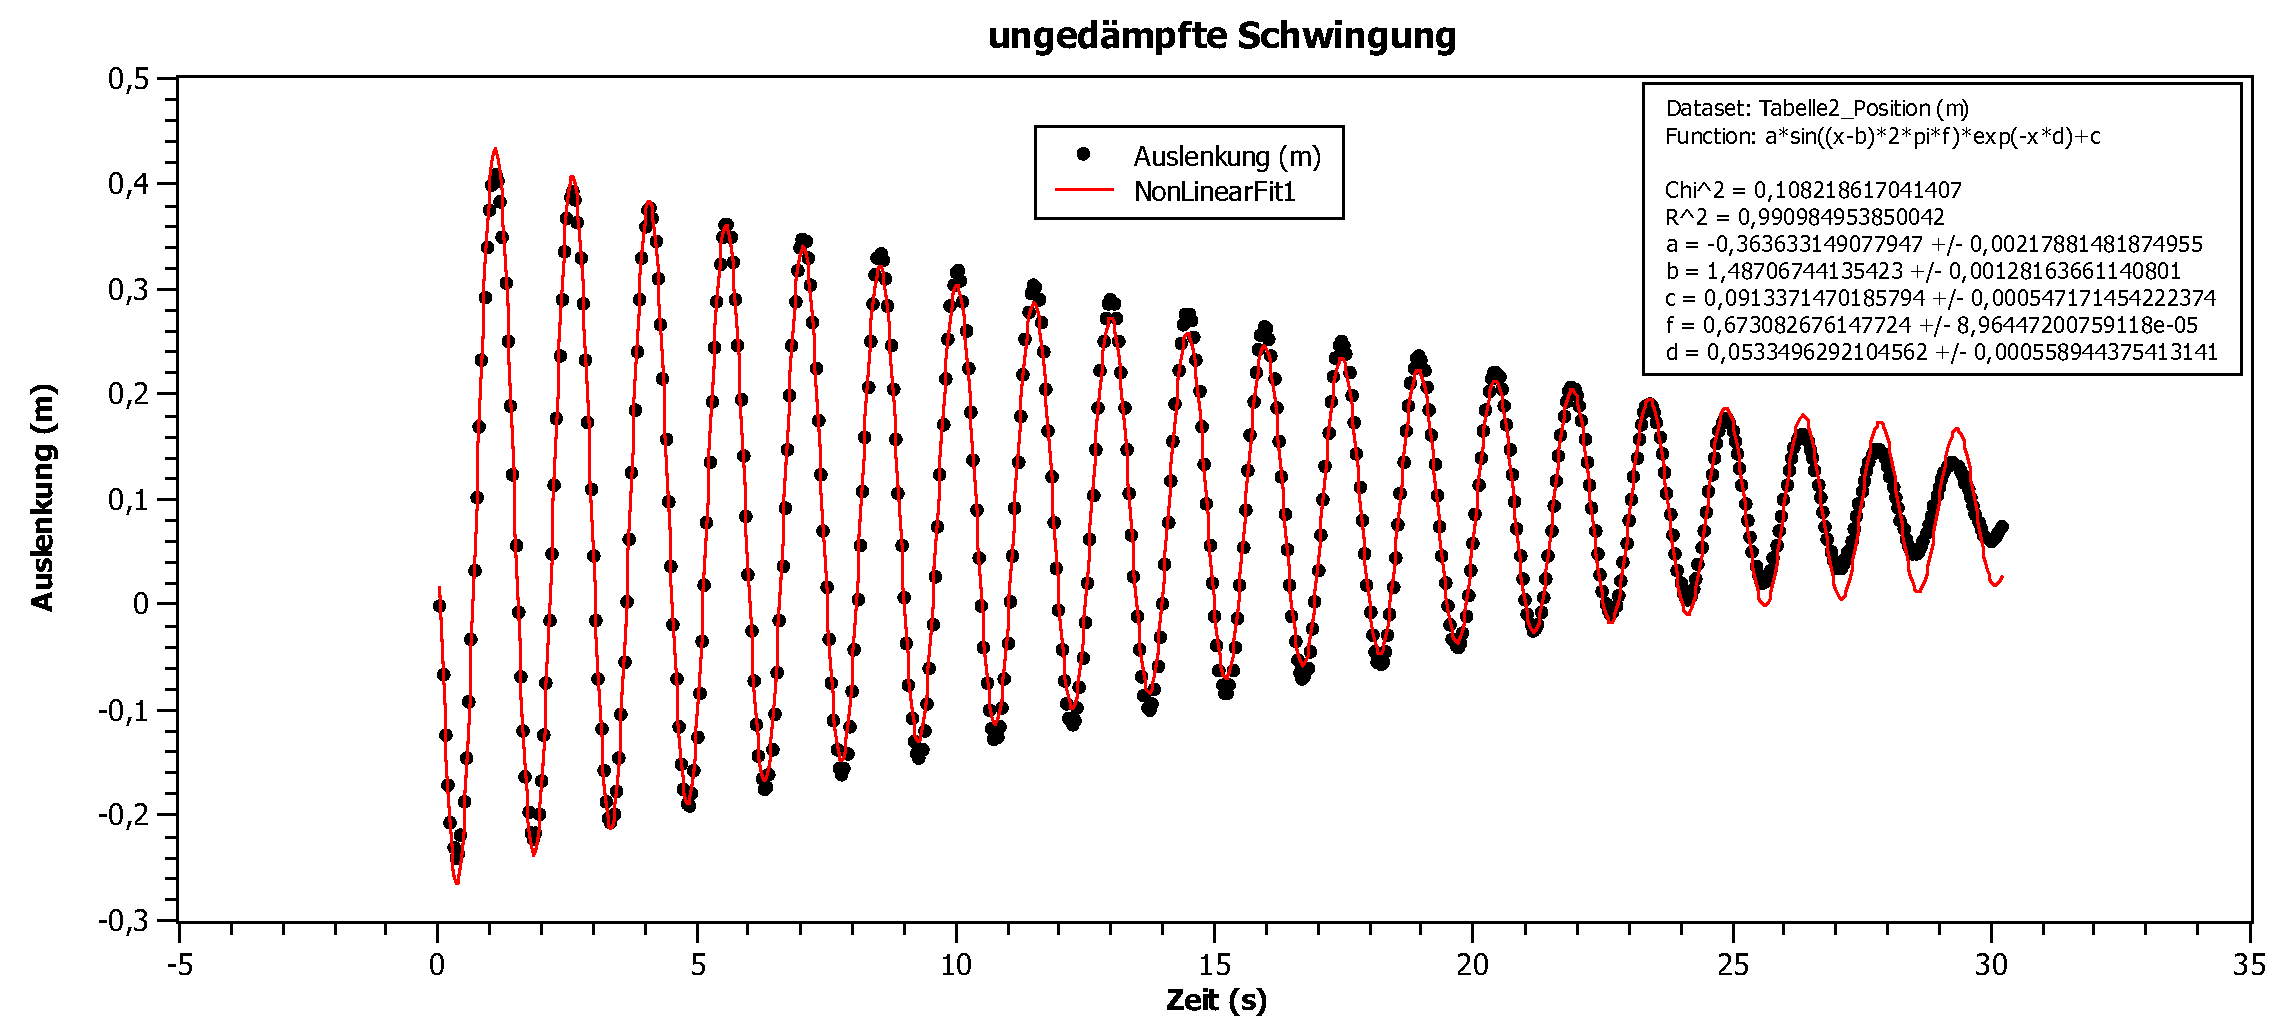
\includegraphics[width=1\textwidth]{Ungedaempfte_Schwingung_Graph}
		\centering
		\caption{Das Ergebnis der mit dem Computer aufgezeichneten Messkurve für die ungedämpfte Schwingung}
		\label{ungedämpfte_Schwingung}
		\centering
	\end{figure}
	In \cref{ungedämpfte_Schwingung} wurden die Messergebnisse der (näherungsweise) ungedämpften Schwingung aufgetragen. Dann wurde ein Fit gemäß dem \enquote{Scaled Levenberg-Marquardt algorithm} mit einer zugrunde liegenden Funktion
	\begin{equation}
	a \sin ((x-b)2 \pi f) \exp^{-x \cdot b} + c
	\end{equation}
	
	durchgeführt.\\
	Dieser ergibt für die Frequenz $ f = \SI{0,67308 \pm 0,00009}{\per \second} $. Dies ist eine rein statistische Unsicherheitsangabe. Zusätzlich entsteht eine Unsicherheit durch ein mögliches Mitrutschen des Seils an beiden Scheiben und die Unsicherheit des Messgerätes. %TODO Ja und wie sind die? cmon pls
	Außerdem lässt sich anhand des Diagramms erkennen (und an der aus dem Fit folgenden Dämpfung $ d= \SI{0,05}{\per \second} $), dass die Annahme, die Schwingung sei ungedämpft, recht unpräzise ist.
	
	\subsection{Drehpendel mit Dämpfung}
	
	Eine Durchführung desselben Fits für die Messungen mit einer Wirbelstrombremse, durch die ein Strom $ I $ fließt, liefert folgendes Ergebnis für die Frequenz $ f $ und die Dämpfung $ d $:\\
	\begin{table}[h]
		\centering
		\begin{tabular}{ r | c | c | c |}
			$I /\si{\ampere}$& 0,2 & 0,3 & 0,5\\ \hline
			$f  /\si{\per \second}$ & 0,67 & 0,67 & 0,67\\
			$d /\si{\per \meter}  $ & 0,11 & 0,16 & 0,34
		\end{tabular}
		\caption{Ergebnisse der Messung der Frequenz $ f $ und der Dämpfung $ d $ bei unterschiedlichen Stromstärken der Wirbelstrombremse}
	\end{table}
	
	\section{Schlussfolgerung}
	
	%\printbibliography
\end{document}
